\section{Auswertung}
\label{sec:Auswertung}

\begin{figure}
  \centering
  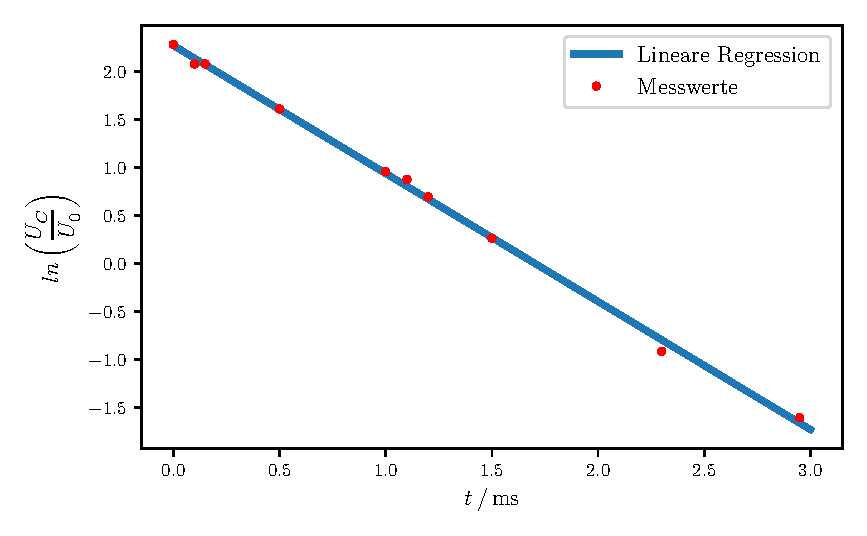
\includegraphics{plot.pdf}
  \caption{Plot.}
  \label{fig:plot}
\end{figure}


Siehe \autoref{fig:plot}!

\begin{table}[H]
\normalsize

\centering
\sisetup{table-format=4.0}
\begin{tabular}{c c c c c c c}
\toprule
        Messung & $U_G \,/\,\si{\volt}$ & $U_C \,/\,\si{\volt}$ & $Frequenz \,/\,\si{\hertz}$ & $a\,/\, \si{\milli\second}$ & $b\,/\, \si{\milli\second}$ & $Phase$ \\
        \midrule
        1   & 5 & 4.9 & 10 & 0.6 & 98 & 574 \\
        2   & 5 & 4.9 & 20 & 1.0 & 50 & 574 \\
        3   & 5 & 4.8 & 30  & 0.8 & 33 & 574 \\ 
        4   & 5 & 4.8 & 40 & 0.76 & 25 & 574 \\
        5   & 5 & 4.8 & 50 & 0.8 & 20 & 574 \\
        6   & 5 & 4.7 & 60 & 0.7 & 16.5 & 574 \\
        7   & 5 & 4.6 & 70 & 0.8 & 14 & 574 \\
        8   & 5 & 4.5 & 80 & 0.8 & 12.4 & 574 \\
        9   & 5 & 4.4 & 90 & 0.8 & 11.2 & 574 \\
        10  & 5 & 4.4 & 100 & 0.7 & 10 & 574 \\
        11  & 5 & 4.2 & 125 & 0.7 & 8 & 574 \\
        12  & 5 & 4.0 & 150 & 0.65 & 6.6 & 574 \\
        13  & 5 & 3.6 & 175 & 0.6 & 5.7 & 574 \\
        14  & 5 & 3.5 & 200 & 0.6 & 5 & 574 \\
        15  & 5 & 2.6 & 300 & 0.5 & 3.3 & 574 \\
        16  & 5 & 2.2 & 400 & 0.4 & 2.5 & 574 \\
        17  & 5 & 1.8 & 500 & 0.4 & 2 & 574 \\
        18  & 5 & 1.2 & 750 & 0.28 & 1.35 & 574 \\
        19  & 5 & 0.95 & 1000 & 0.2 & 1 & 574 \\
        20  & 5 & 0.20 & 5000 & 0.05 & 0.2 & 574 \\
        21  & 5 & 0.10& 10000 & 0.025 & 0.1 & 574 \\



        
\bottomrule

\end{tabular}

\caption{Aufgenommene Werte zur Bestimmung von $R_{11}$}
\label{tab:1}
\end{table}